\chapter{The projective plane}\label{chapter:projective.plane}%
\section{Homogenizing}
Take a cubic polynomial
\[
p(x)=ax^3+bx^2+cx+d.
\]
Associate to it the homogeneous polynomial in two variables
\[
P(x,y)=ax^3+bx^2y+cxy^2+dy^3
\]
by sticking in a power of \(y\) in each term so that the term reaches degree \(3\) in \(x\) and \(y\) together.
The original polynomial is \(p(x)=P(x,1)\), i.e. set \(y=1\).
So geometrically, \(p(x)\) is just \(P(x,y)\) but only calculated along the line \(y=1\).
\begin{problem}{projective.plane:homog}
Homogenize \(p(x)=x^4+x+1\).
\end{problem}
\begin{answer}{projective.plane:homog}
\(P(x,y)=x^4+xy^3+y^4\)
\end{answer}
\begin{problem}{projective.plane:homogenise}
Homogenise \(x^2y - x^2 + y = 1 + 2x - y^2x^3\), sticking in a new variable \(z\).
\end{problem}
In sage:
\begin{sageblock}
R.<x,y,z> = PolynomialRing(QQ)
p = x^3+x*y+1
p.homogenize(z)
\end{sageblock}
yields \(\sage{p.homogenize(z)}\).
All terms have degree \(3\) so, when we rescale the variables, every term scales by \(3\) factors of the scaling
\[
P(sx,sy)=s^3P(x,y)
\]
In particular, if \(P(x,y)\) vanishes at some point \((x,y)=(x_0,y_0)\) of the plane, it also vanishes at every rescaling of that point.
So it also vanishes on the line through \((x_0,y_0)\) and \((0,0)\).
Thus the zeroes of a homogeneous polynomial form a collection of lines through the origin.
\begin{example}
Taking \(p(x)=x(x-1)(x+1)\), we find
\[
P(x,y)=x(x-y)(x+y)
\]
by making each factor homogeneous.
On the graph of \(P(x,y)\) we see the graph of \(p(x)\) along the line \(y=1\):
\begin{center}
\documentclass{standalone}
\usepackage{pgfplots}
\pgfplotsset{width=7cm,compat=1.17}
\usepgfplotslibrary{fillbetween}
\begin{document}
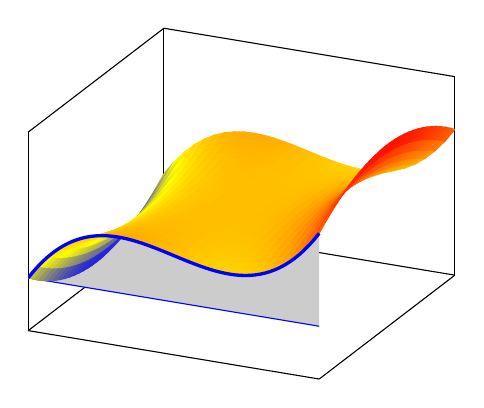
\begin{tikzpicture}
\begin{axis}[
%height=15cm,
%hide axis,
%axis lines=center,
%axis on top,
%axis line style={draw=none},
%tick style={draw=none},
xtick=\empty,
ytick=\empty,
ztick=\empty,
]
\newcommand{\xxx}{1.51}
\newcommand{\rrr}{-1}
\addplot3+[name path=A,blue,domain=-\xxx:\xxx,samples=60,samples y=0,mark=none] 
		({x},
		 {-1},
		 {20*(-\xxx)*(-\xxx-\rrr)*(-\xxx-1)});
\addplot3 [
surf,
shader=flat,
%faceted color=gray,
samples=30,
domain=-\xxx:\xxx,y domain=-1:1
] {20*x*(x+y)*(x+\rrr*y)};
\addplot3+[name path=B,blue,very thick,domain=-\xxx:\xxx,samples=60,samples y=0,mark=none] 
		({x},
		 {-1},
		 {20*x*(x-\rrr)*(x-1)});
\addplot3[gray!40] fill between[of=A and B];
%\addplot3+[black,thick,domain=-1:1,samples=60,samples y=0,mark=none] 
%		({0},
%		 {x},
%		 {0});
%\addplot3+[black,thick,domain=-1:1,samples=60,samples y=0,mark=none] 
%		({-x},
%		 {x},
%		 {0});
%\addplot3+[black,thick,domain=-1:1,samples=60,samples y=0,mark=none] 
%		({-\rrr*x},
%		 {x},
%		 {0});
\end{axis}
\end{tikzpicture}
\end{document}
\end{center}
So \(P(x,y)\) vanishes on the lines \(x=0\), \(x=y\), \(x=-y\) in the plane.
These lines intersect the line \(y=1\) at \(x=0\), \(x=1\), \(x=-1\), the roots of \(p(x)\).
\begin{center}
\documentclass{standalone}
\usepackage{pgfplots}
\pgfplotsset{width=7cm,compat=1.17}
\usepgfplotslibrary{fillbetween}
\NewDocumentCommand\DrawDotThreeD{O{}mmmO{}}%
{%
\fill[gray!20,draw=gray] ({#2},{#3},{#4}) circle (1.6pt) node[above,black,#5] {\(#1\)};%
}%
\begin{document}
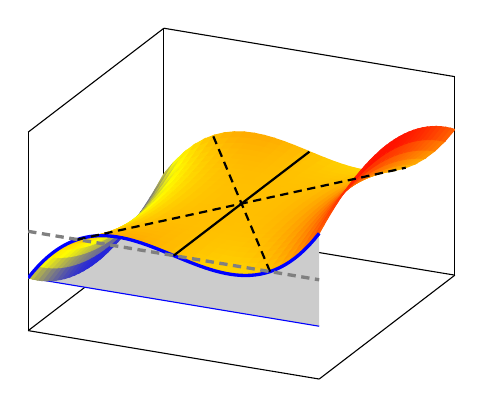
\begin{tikzpicture}
\begin{axis}[
%height=15cm,
%hide axis,
%axis lines=center,
%axis on top,
%axis line style={draw=none},
%tick style={draw=none},
xtick=\empty,
ytick=\empty,
ztick=\empty,
]
\newcommand{\xxx}{1.51}
\newcommand{\rrr}{-1}
\addplot3+[name path=A,blue,domain=-\xxx:\xxx,samples=60,samples y=0,mark=none] 
		({x},
		 {-1},
		 {20*(-\xxx)*(-\xxx-\rrr)*(-\xxx-1)});
\addplot3 [
surf,
shader=flat,
%faceted color=gray,
samples=30,
domain=-\xxx:\xxx,y domain=-1:1
] {20*x*(x+y)*(x+\rrr*y)};
\addplot3+[name path=B,blue,very thick,domain=-\xxx:\xxx,samples=60,samples y=0,mark=none] 
		({x},
		 {-1},
		 {20*x*(x-\rrr)*(x-1)});
\addplot3[gray!40] fill between[of=A and B];
\addplot3+[black,thick,domain=-1:1,samples=60,samples y=0,mark=none] 
		({0},
		 {x},
		 {0});
\addplot3+[black,thick,domain=-1:1,samples=60,samples y=0,mark=none] 
		({-x},
		 {x},
		 {0});
\addplot3+[black,thick,domain=-1:1,samples=60,samples y=0,mark=none] 
		({-\rrr*x},
		 {x},
		 {0});
\addplot3+[gray,very thick,domain=-\xxx:\xxx,samples=60,samples y=0,mark=none] 
		({x},
		 {-1},
		 {0});
\DrawDotThreeD{0}{-1}{0}
\DrawDotThreeD{1}{-1}{0}
\DrawDotThreeD{-1}{-1}{0}
\end{axis}
\end{tikzpicture}
\end{document}
\end{center}
\end{example}
\begin{problem}{projective.plane:homog.2}
Starting with \(p(x)=x^3+x\), compute \(P(x,y)\), find the real roots of \(p(x)\) and the lines through the origin on which \(P(x,y)\) vanishes.
Draw the graph of \(P(x,y)\); indicate on it where the graph of \(p(x)\) lies.
\end{problem}
Passing from the polynomial \(p(x)\) to the homogeneous polynomial \(P(x,y)\), we lose no information, since \(p(x)=P(x,1)\).
The same trick works for polynomials of any degree.
\begin{problem}{projective.plane:homog.3}
Prove that the homogeneous polynomial \(P(x,y)\) associated as above to a polynomial \(p(x)\) is the unique homogeneous polynomial that agrees with \(p(x)\) along the line \(y=1\).
\end{problem}
If we like we can even pick a polynomial \(p(x)\) of some degree and homogenize it to a polynomial \(P(x,y)\) of some higher degree, sticking in as many \(y\) factors as needed into each term:
\begin{example}
The polynomial \(p(x)=x(x-1)\) has degree \(2\), but think of it as a ``degenerate'' degree \(4\) polynomial, so homogenize to \(P(x,y)=x(x-y)y^2\), adding in any extra two \(y\) factors to reach degree \(4\).
We will soon see that we can think of \(p(x)\) as a quartic polynomial with ``two roots at infinity''.
\end{example}
\section{Watch a moving root}
A cubic polynomial in one variable might have three roots:
\begin{center}
\documentclass[tikz]{standalone}
\usepackage{pgfplots}
\colorlet{curveZero}{gray!85}
\colorlet{curveOne}{blue!60}
\definecolor{curveOneColor}{rgb}{.6,0,0}
\colorlet{curveTwo}{brown!50!gray}
\colorlet{curveThree}{green!40!gray}
\colorlet{curveFour}{red!50!gray}
\NewDocumentCommand\DrawDotInPlot{O{}mmO{}}%
{%
\fill[gray!15,draw=gray] (axis cs:{#2},{#3}) circle [radius=1.6pt] node[above,black,#4] {\(#1\)};%
}%
\NewDocumentCommand\DrawDot{O{}mmO{}}%
{%
\fill[gray!20,draw=gray] ({#2},{#3}) circle (1.6pt) node[above,black,#4] {\(#1\)};%
}%
\NewDocumentCommand\DrawNode{O{}m}%
{%
\fill[gray!20,draw=gray] (#2) circle (1.6pt) node[above,black] {\(#1\)};%
}%
\NewDocumentCommand\DrawDotThreeD{O{}mmmO{}}%
{%
\fill[gray!20,draw=gray] ({#2},{#3},{#4}) circle (1.6pt) node[above,black,#5] {\(#1\)};%
}%
\colorlet{axisColor}{gray!50}
\tikzstyle{shapeZero}=[fill=curveZero,opacity=.4]
\tikzstyle{shapeOne}=[fill=curveOne,opacity=.4]
\tikzstyle{shapeTwo}=[fill=curveTwo,opacity=.4]
\tikzstyle{shapeThree}=[fill=curveThree,opacity=.4]
\tikzstyle{groupElementLabel}=[minimum size=2.4em]
\tikzstyle{groupElement}=[minimum size=2.4em,shapeZero,draw=curveZero]
\tikzstyle{cosetOne}=[minimum size=2.4em,shapeOne,draw=curveOne]
\tikzstyle{cosetTwo}=[minimum size=2.4em,shapeTwo,draw=curveTwo]


\begin{document}
\begin{tikzpicture}
\draw[curveZero] (-1.2,0) -- (1.2,0);
\draw[very thick,curveOne,domain=-1.2:1.2] plot (\x,{\x*(\x-1)*(\x+1)});
%\draw[very thick,curveTwo,domain=-1:1] plot (\x,{-.5*\x*\x*\x});
\DrawDot{0}{0}
\DrawDot{-1}{0}
\DrawDot{1}{0}
%\fill[curveOne] (0,0) circle (2pt);
%\fill[curveOne] (-1,0) circle (2pt);
%\fill[curveOne] (1,0) circle (2pt);
%\draw[very thick,curveThree,domain=-1:1] plot (\x,{-1+.25*\x*\x*\x});
\end{tikzpicture}
\end{document}
\end{center}
We can put them wherever we like by picking suitable coefficients.
Imagine one of them moves far away, so at time \(t\), we want our roots to be at \(x=0,x=1,x=t\).
We could pick the polynomial to be \(x(x-1)(x-t)\); but this has no limit as \(t\) gets large, 
since there is a factor of \(t\) in our polynomial.
Fix this: divide out by \(t\), say take our polynomial to be instead \(x(x-1)(x-t)/t\), which does not change the roots.
Expand this out:
\[
\frac{x(x-1)(x-t)}{t}=\frac{x^3}{t}-\left(1+\frac{1}{t}\right)x^2+x.
\]
For nonzero \(t\), the coefficients remain bounded as \(t\) gets large.
\begin{center}
\documentclass[tikz]{standalone}
\usepackage{pgfplots}
\colorlet{curveZero}{gray!85}
\colorlet{curveOne}{blue!60}
\definecolor{curveOneColor}{rgb}{.6,0,0}
\colorlet{curveTwo}{brown!50!gray}
\colorlet{curveThree}{green!40!gray}
\colorlet{curveFour}{red!50!gray}
\NewDocumentCommand\DrawDotInPlot{O{}mmO{}}%
{%
\fill[gray!15,draw=gray] (axis cs:{#2},{#3}) circle [radius=1.6pt] node[above,black,#4] {\(#1\)};%
}%
\NewDocumentCommand\DrawDot{O{}mmO{}}%
{%
\fill[gray!20,draw=gray] ({#2},{#3}) circle (1.6pt) node[above,black,#4] {\(#1\)};%
}%
\NewDocumentCommand\DrawNode{O{}m}%
{%
\fill[gray!20,draw=gray] (#2) circle (1.6pt) node[above,black] {\(#1\)};%
}%
\NewDocumentCommand\DrawDotThreeD{O{}mmmO{}}%
{%
\fill[gray!20,draw=gray] ({#2},{#3},{#4}) circle (1.6pt) node[above,black,#5] {\(#1\)};%
}%
\colorlet{axisColor}{gray!50}
\tikzstyle{shapeZero}=[fill=curveZero,opacity=.4]
\tikzstyle{shapeOne}=[fill=curveOne,opacity=.4]
\tikzstyle{shapeTwo}=[fill=curveTwo,opacity=.4]
\tikzstyle{shapeThree}=[fill=curveThree,opacity=.4]
\tikzstyle{groupElementLabel}=[minimum size=2.4em]
\tikzstyle{groupElement}=[minimum size=2.4em,shapeZero,draw=curveZero]
\tikzstyle{cosetOne}=[minimum size=2.4em,shapeOne,draw=curveOne]
\tikzstyle{cosetTwo}=[minimum size=2.4em,shapeTwo,draw=curveTwo]


\begin{document}
\begin{tikzpicture}
\draw[curveZero] (-1,0) -- (1.5,0);
%\draw[very thick,curveTwo,domain=-1:1] plot (\x,{-.5*\x*\x*\x});
%\fill[curveOne] (0,0) circle (2pt);
%\fill[curveOne] (-.8,0) circle (2pt);
\foreach \i/\j in {.8/10,1/20,1.2/30,1.4/40,1.6/50,1.8/60,2/70,2.2/80,2.4/90,2.6/100}
{
	\draw[very thick,curveOne!\j!curveTwo,domain=-1:1.5] plot (\x,{\x*(\x/\i-1)*(\x+.8)});
}
\DrawDot{0}{0}
\DrawDot{-.8}{0}
%\draw[very thick,curveTwo,domain=-1:1.5] plot (\x,{\x*(-1)*(\x+.8)});
%\fill[curveOne] (.8,0) circle (2pt);
%\draw[very thick,curveThree,domain=-1:1] plot (\x,{-1+.25*\x*\x*\x});
\end{tikzpicture}
\end{document}
\end{center}
So our root moves far away, while the coefficients remain bounded.
What happens as \(t\) becomes infinite?
\begin{center}
\documentclass[tikz]{standalone}
\usepackage{pgfplots}
\colorlet{curveZero}{gray!85}
\colorlet{curveOne}{blue!60}
\definecolor{curveOneColor}{rgb}{.6,0,0}
\colorlet{curveTwo}{brown!50!gray}
\colorlet{curveThree}{green!40!gray}
\colorlet{curveFour}{red!50!gray}
\NewDocumentCommand\DrawDotInPlot{O{}mmO{}}%
{%
\fill[gray!15,draw=gray] (axis cs:{#2},{#3}) circle [radius=1.6pt] node[above,black,#4] {\(#1\)};%
}%
\NewDocumentCommand\DrawDot{O{}mmO{}}%
{%
\fill[gray!20,draw=gray] ({#2},{#3}) circle (1.6pt) node[above,black,#4] {\(#1\)};%
}%
\NewDocumentCommand\DrawNode{O{}m}%
{%
\fill[gray!20,draw=gray] (#2) circle (1.6pt) node[above,black] {\(#1\)};%
}%
\NewDocumentCommand\DrawDotThreeD{O{}mmmO{}}%
{%
\fill[gray!20,draw=gray] ({#2},{#3},{#4}) circle (1.6pt) node[above,black,#5] {\(#1\)};%
}%
\colorlet{axisColor}{gray!50}
\tikzstyle{shapeZero}=[fill=curveZero,opacity=.4]
\tikzstyle{shapeOne}=[fill=curveOne,opacity=.4]
\tikzstyle{shapeTwo}=[fill=curveTwo,opacity=.4]
\tikzstyle{shapeThree}=[fill=curveThree,opacity=.4]
\tikzstyle{groupElementLabel}=[minimum size=2.4em]
\tikzstyle{groupElement}=[minimum size=2.4em,shapeZero,draw=curveZero]
\tikzstyle{cosetOne}=[minimum size=2.4em,shapeOne,draw=curveOne]
\tikzstyle{cosetTwo}=[minimum size=2.4em,shapeTwo,draw=curveTwo]


\begin{document}
\begin{tikzpicture}
\draw[curveZero] (-1,0) -- (1.5,0);
%\draw[very thick,curveTwo,domain=-1:1] plot (\x,{-.5*\x*\x*\x});
%\fill[curveOne] (0,0) circle (2pt);
%\fill[curveOne] (-.8,0) circle (2pt);
\foreach \i/\j in {.8/10,1/20,1.2/30,1.4/40,1.6/50,1.8/60,2/70,2.2/80,2.4/90,2.6/100}
{
	\draw[very thick,curveOne!\j!curveTwo,domain=-1:1.5] plot (\x,{\x*(\x/\i-1)*(\x+.8)});
}
\draw[very thick,curveOne,domain=-1:1.5] plot (\x,{\x*(-1)*(\x+.8)});
\DrawDot{0}{0}
\DrawDot{-.8}{0}
%\fill[curveOne] (.8,0) circle (2pt);
%\draw[very thick,curveThree,domain=-1:1] plot (\x,{-1+.25*\x*\x*\x});
\end{tikzpicture}
\end{document}
\end{center}
Our polynomial reaches a limit
\[
-x^2+x=x(1-x).
\]
The two fixed roots stay in place, but the polynomial drops degree when the moving root disappears to infinity.
\section{Homogenize the moving roots}
While we watch our moving polynomial \(p(x)\), we can also watch its homogenization \(P(x,y)\).
The roots of \(P(x,y)\) behave better as we allow them to move: we picture that the lines only turn around, but they can't disappear, because they continue to pass through the origin.
\begin{example}
Return to our example of 
\[
p(x)=\frac{x(x-1)(x-t)}{t}.
\]
Just think of \(t\) as a constant for now; we will soon let it move.
Homogenize:
\[
P(x,y)=\frac{x(x-y)(x-ty)}{t}.
\]
So the roots are the lines \(x=0\), \(x=y\), \(x=ty\).
As we let \(t\) get large, the line \(x=ty\) can be written as \(x/t=y\), so becomes \(0=y\) in the limit.
\end{example}
Take any polynomial \(p_t(x)\) whose coefficients depend on some parameter \(t\) (or maybe several parameters).
Imagine we compute out the associated homogeneous polynomial, call it \(P_t(x,y)\).
Suppose that \(p_t(x)\) has some degree \(d\), except maybe for certain ``special'' values of \(t\).
As long as the coefficients of \(p_t(x)\) don't all disappear at once, i.e. for the same value of \(t\) or limit of \(t\), the same is true of \(P_t(x,y)\), since they are the same coefficients.
All terms in the homogeneous polynomial \(P_t(x,y)\) have degree exactly \(d\).
Since they never all vanish, \(P_t(x,y)\) doesn't drop degree for any value or limit of \(t\).
\section{The projective line}
When we homogenize a polynomial, each point \(x\) becomes a unique point \((x,y)=(x,1)\) on the line \(y=1\).
\begin{center}
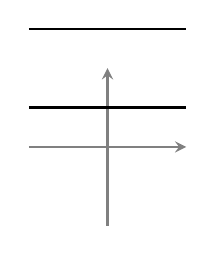
\begin{tikzpicture}
\draw[black,thick] (-1,1.5) -- (1,1.5);
\DrawDot{-.6}{1.5}
%\fill[black] (-1.2,3) circle (3pt);
\draw[gray,thick,-stealth] (-1,0) -- (1,0);
\draw[gray,thick,-stealth] (0,-1) -- (0,1);
\draw[black,thick] (-1,.5) -- (1,.5);
\DrawDot{-.6}{.5}
%\fill[black] (-1.2,1) circle (3pt);
\end{tikzpicture}
\end{center}
Conversely, each point \((x,y)=(x,1)\) arises in this way from a point \(x\).
But each point \((x,1)\) also spans a line through the origin.
\begin{center}
\begin{tikzpicture}
\draw[gray,thick,-stealth] (-1,0) -- (1,0);
\draw[gray,thick,-stealth] (0,-1) -- (0,1);
\draw[black,thick] (-1,.5) -- (1,.5);
\draw[curveOne,very thick] (-1,{5/6}) -- (1,{-5/6});
\DrawDot{-.6}{.5}
%\fill[black] (-1.2,1) circle (3pt);
\DrawDot{0}{0}
%\fill[curveOne] (0,0) circle (3pt);
\end{tikzpicture}
\end{center}
Every line through the origin arises uniquely in this way except \(y=0\), which we can think of as \(x=\infty\).
Spin the line around the origin.
\begin{center}
\documentclass[tikz]{standalone}
\colorlet{curveZero}{gray!85}
\colorlet{curveOne}{blue!60}
\definecolor{curveOneColor}{rgb}{.6,0,0}
\colorlet{curveTwo}{brown!50!gray}
\colorlet{curveThree}{green!40!gray}
\colorlet{curveFour}{red!50!gray}
\NewDocumentCommand\DrawDotInPlot{O{}mmO{}}%
{%
\fill[gray!15,draw=gray] (axis cs:{#2},{#3}) circle [radius=1.6pt] node[above,black,#4] {\(#1\)};%
}%
\NewDocumentCommand\DrawDot{O{}mmO{}}%
{%
\fill[gray!20,draw=gray] ({#2},{#3}) circle (1.6pt) node[above,black,#4] {\(#1\)};%
}%
\NewDocumentCommand\DrawNode{O{}m}%
{%
\fill[gray!20,draw=gray] (#2) circle (1.6pt) node[above,black] {\(#1\)};%
}%
\NewDocumentCommand\DrawDotThreeD{O{}mmmO{}}%
{%
\fill[gray!20,draw=gray] ({#2},{#3},{#4}) circle (1.6pt) node[above,black,#5] {\(#1\)};%
}%
\colorlet{axisColor}{gray!50}
\tikzstyle{shapeZero}=[fill=curveZero,opacity=.4]
\tikzstyle{shapeOne}=[fill=curveOne,opacity=.4]
\tikzstyle{shapeTwo}=[fill=curveTwo,opacity=.4]
\tikzstyle{shapeThree}=[fill=curveThree,opacity=.4]
\tikzstyle{groupElementLabel}=[minimum size=2.4em]
\tikzstyle{groupElement}=[minimum size=2.4em,shapeZero,draw=curveZero]
\tikzstyle{cosetOne}=[minimum size=2.4em,shapeOne,draw=curveOne]
\tikzstyle{cosetTwo}=[minimum size=2.4em,shapeTwo,draw=curveTwo]


\begin{document}
\begin{tikzpicture}
\draw[gray,thick,-stealth] (-1,0) -- (1,0);
\draw[gray,thick,-stealth] (0,-1) -- (0,1);
\draw[black,thick] (-1,.5) -- (1,.5);
\begin{scope}
    \clip(-1,-1) rectangle (1,1);
	\foreach \i in {1,...,7}
	{
		\pgfmathsetmacro\clr{100-5*\i}
		\pgfmathsetmacro\thet{130-15*\i}
		\draw[draw=curveOne!\clr,very thick] ({2*cos(\thet)},{2*sin(\thet)}) -- ({-2*cos(\thet)},{-2*sin(\thet)});
		\pgfmathsetmacro\xxx{cot(\thet)/2}
		\DrawDot{\xxx}{.5}
	}
\end{scope}
\DrawDot{0}{0}
\end{tikzpicture}
\end{document}
\end{center}
As we spin, our line strikes \(y=1\) at some point \((x,1)\), which we think of as a number \(x\); picture the line spinning clockwise, so \(x\to\infty\).
When our spinning line becomes horizontal, it becomes \(y=0\), so \(x=\infty\).
After that, as the angle of the line goes further around clockwise, we now find it strikes a point \((x,1)\) of our line \(y=1\) but with \(x<0\).
So we have ``passed through infinity'' and found ourselves wrapping around to negative numbers:
\begin{center}
\documentclass[tikz]{standalone}
\colorlet{curveZero}{gray!85}
\colorlet{curveOne}{blue!60}
\definecolor{curveOneColor}{rgb}{.6,0,0}
\colorlet{curveTwo}{brown!50!gray}
\colorlet{curveThree}{green!40!gray}
\colorlet{curveFour}{red!50!gray}
\NewDocumentCommand\DrawDotInPlot{O{}mmO{}}%
{%
\fill[gray!15,draw=gray] (axis cs:{#2},{#3}) circle [radius=1.6pt] node[above,black,#4] {\(#1\)};%
}%
\NewDocumentCommand\DrawDot{O{}mmO{}}%
{%
\fill[gray!20,draw=gray] ({#2},{#3}) circle (1.6pt) node[above,black,#4] {\(#1\)};%
}%
\NewDocumentCommand\DrawNode{O{}m}%
{%
\fill[gray!20,draw=gray] (#2) circle (1.6pt) node[above,black] {\(#1\)};%
}%
\NewDocumentCommand\DrawDotThreeD{O{}mmmO{}}%
{%
\fill[gray!20,draw=gray] ({#2},{#3},{#4}) circle (1.6pt) node[above,black,#5] {\(#1\)};%
}%
\colorlet{axisColor}{gray!50}
\tikzstyle{shapeZero}=[fill=curveZero,opacity=.4]
\tikzstyle{shapeOne}=[fill=curveOne,opacity=.4]
\tikzstyle{shapeTwo}=[fill=curveTwo,opacity=.4]
\tikzstyle{shapeThree}=[fill=curveThree,opacity=.4]
\tikzstyle{groupElementLabel}=[minimum size=2.4em]
\tikzstyle{groupElement}=[minimum size=2.4em,shapeZero,draw=curveZero]
\tikzstyle{cosetOne}=[minimum size=2.4em,shapeOne,draw=curveOne]
\tikzstyle{cosetTwo}=[minimum size=2.4em,shapeTwo,draw=curveTwo]


\begin{document}
\begin{tikzpicture}
\draw (0,0) circle (1cm);
\node[above] at (0,1) {\(0\)};
\node[below] at (0,-1) {\(\infty\)};
\node[left] at (-1,0) {\(-\)};
\node[right] at (1,0) {\(+\)};
\DrawDot{0}{1}
\DrawDot{0}{-1}
\end{tikzpicture}
\end{document}
\end{center}

The \emph{projective line}\define{projective!line}\define{line!projective} \(\Proj^1_k\) of a field \(k\) is the set of all lines through the origin in the plane \(k^2\); each is uniquely expressed as \(x=ty\) for some element \(t\) from \(k\) (and so is naturally thought of as an element \(t\) of \(k\)), except for the line \(y=0\) (which we naturally write as \(t=\infty\)).
Every polynomial \(p(x)\), in one variable \(x\), of degree at most some positive integer \(d\), is naturally identified with a homogeneous polynomial \(P(x,y)\) of degree exactly \(d\), which then has roots in the projective line; to make sense of this, we must fix the choice of \(d\), some integer which is at least as large as the actual degree of \(p(x)\).
If \(p(x)\) has degree less than \(d\), say some degree \(d_0\), we can treat that as meaning that \(P(x,y)\) has \(d-d_0\) factors of \(y\), or say that \(p(x)\) has \(d-d_0\) ``roots at infinity''.
We are not afraid to work with roots at infinity, since we can always write out \(P(x,y)\) to make precise what we mean.
Roots won't disappear as we vary the coefficients of \(p(x)\), when we compute roots in the projective line; they only move to infinity, or even move across infinity.
We are forced to look for our roots on the projective line whenever we have a polynomial whose coefficients vary with some parameter.
\begin{problem}{projective.plane:lin.frac}
Suppose that we change variables \(x,y\) by a linear transformation, say to
\[
\begin{pmatrix}
X\\
Y
\end{pmatrix}
=
A
\begin{pmatrix}
x\\
y
\end{pmatrix}
\]
where
\[
A=
\begin{pmatrix}
a&b\\
c&d
\end{pmatrix}.
\]
Show that the line \(x=ty\) changes to the line \(X=TY\) given by the associated \emph{projective transformation}\define{projective!transformation}
\[
T=\frac{at+b}{ct+d}.
\]
\end{problem}

\section{The projective plane}
\epigraph[author={Arthur Cayley}]{The more systematic course in the present introductory memoir \dots
would have been to ignore altogether the notions of distance and
metrical geometry \dots. Metrical geometry is a part of descriptive
geometry, and descriptive geometry is all geometry.}\SubIndex{Cayley, Arthur}%
The old fashioned term \emph{descriptive geometry}\define{descriptive geometry} means the geometry of straight lines.
Straight lines in the plane remain straight when you rescale the plane, or translate the plane to the left or right, up or down, or when you rotate the plane.
They even remain straight when you carry out any linear change of variables, as you know from linear algebra.

\bigskip

\epigraph[author={William Blake}, source={Auguries of Innocence}]{To see a World in a Grain of Sand, \\ And Heaven in a Wild Flower. \\ Hold Infinity in the palm of your hand, \\ And Eternity in an hour.}\SubIndex{Blake, William}%
Railway tracks built on a flat plane appear to meet ``at infinity''.
\begin{center}
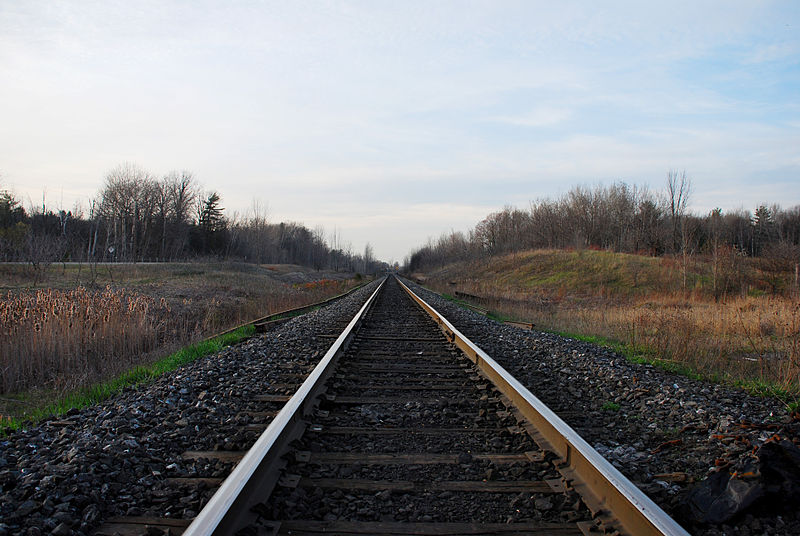
\includegraphics[width=4cm]{railway-tracks.jpg} \\[2pt]
\begin{minipage}{4cm}\raggedright\tiny{Creative Commons Attribution-Share Alike 3.0 Unported license. I, MarcusObal}\end{minipage}
\end{center}
Imagine that we were to add a point to the plane ``at infinity'' in the direction where these tracks (straight lines) appear to meet.
\emph{Danger:} in order to add only one point, imagine that the two rails meet at the \emph{same} point in one direction as they do in the other, making them both into circles.
The projective plane is the set of all of the usual points of the plane (which we can think of as the ``finite points'' of the projective plane) together with some sort of ``points at infinity'' to represent the directions in the plane.

\newpage

\epigraph[author={Fyodor Dostoyevsky}, source={The Brothers Karamazov}]{
But you must note this: if God exists and if He really did
create the world, then, as we all know, He created it according to
the geometry of Euclid and the human mind with the conception
of only three dimensions in space.  Yet there have been and
still are geometricians and philosophers, and even some of the
most distinguished, who doubt whether the whole universe, or
to speak more widely the whole of being, was only created in
Euclid's geometry; they even dare to dream that two parallel
lines, which according to Euclid can never meet on earth, may
meet somewhere in infinity.}\SubIndex{Dostoyevsky, Fyodor}\SubIndex{Brothers Karamazov}


We would like a more precise mathematical definition of points ``at infinity''.
Place yourself at a vantage point above the plane.
\begin{center}
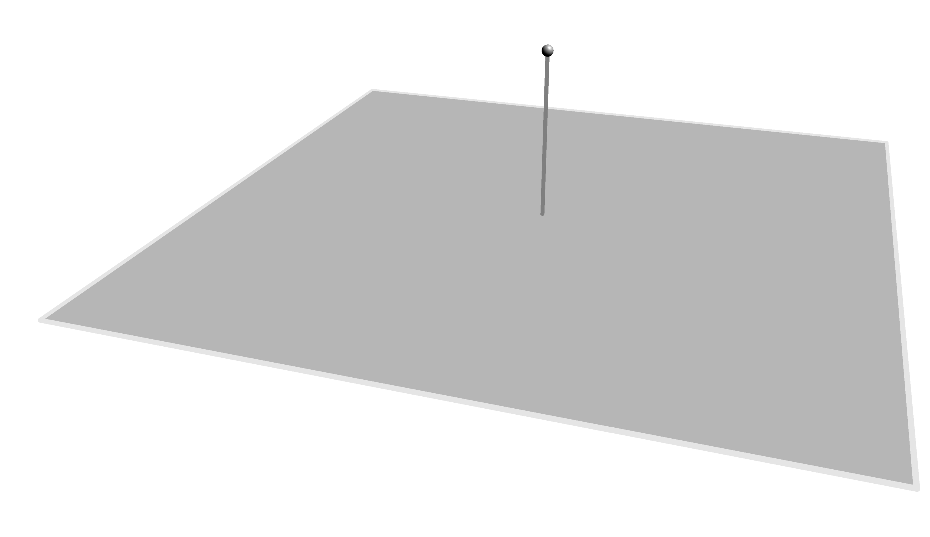
\includegraphics[width=5cm]{above-the-plane-vantage}
\end{center}
Every ``finite'' point of the plane lies on a line through your vantage point: the line of sight.
\begin{center}
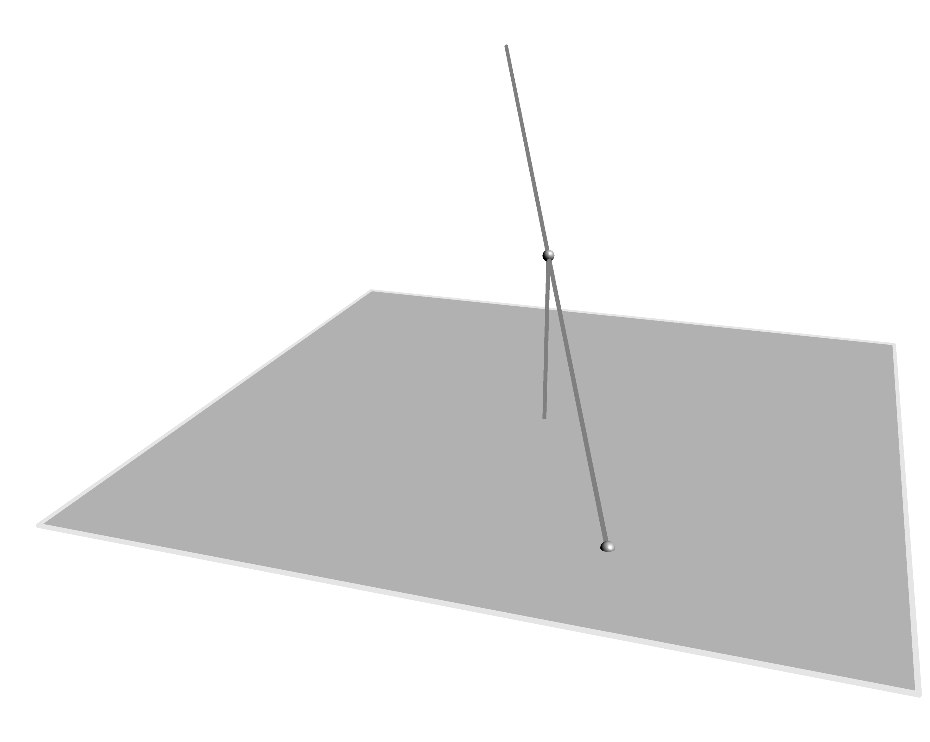
\includegraphics[width=5cm]{above-the-plane-connect}
\end{center}
You can also look out to the points at infinity, along lines:
\begin{center}
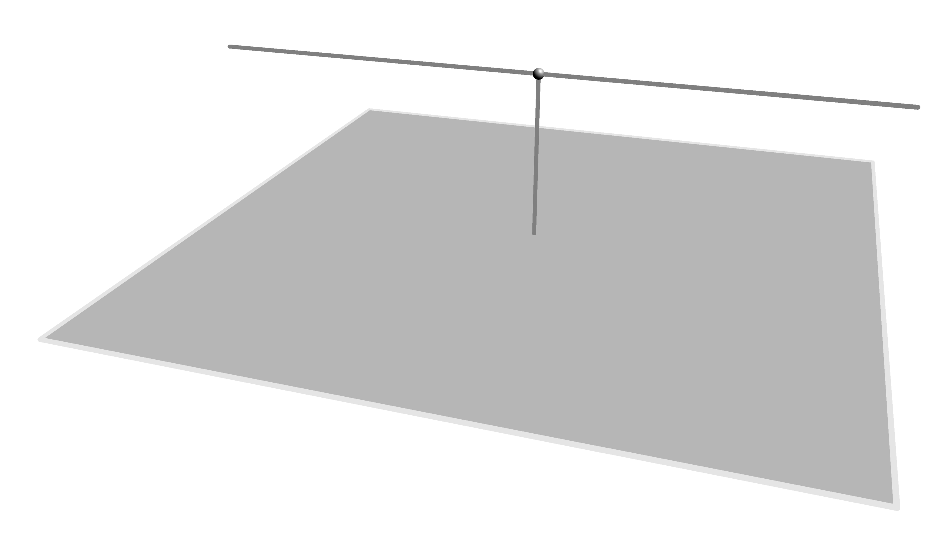
\includegraphics[width=5cm]{above-the-plane-off-to-infinity}
\end{center}
For example, there is such a line  parallel to the lines of our train track:
\begin{center}
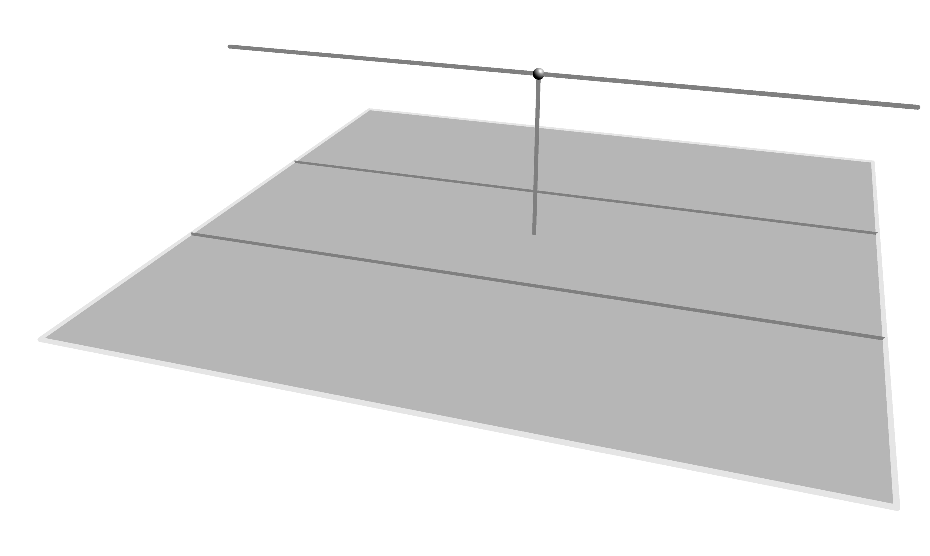
\includegraphics[width=5cm]{above-the-plane-3}
\end{center}

On the other hand, if we take any line through the vantage point, either it hits a ``finite'' point of the plane:
\begin{center}
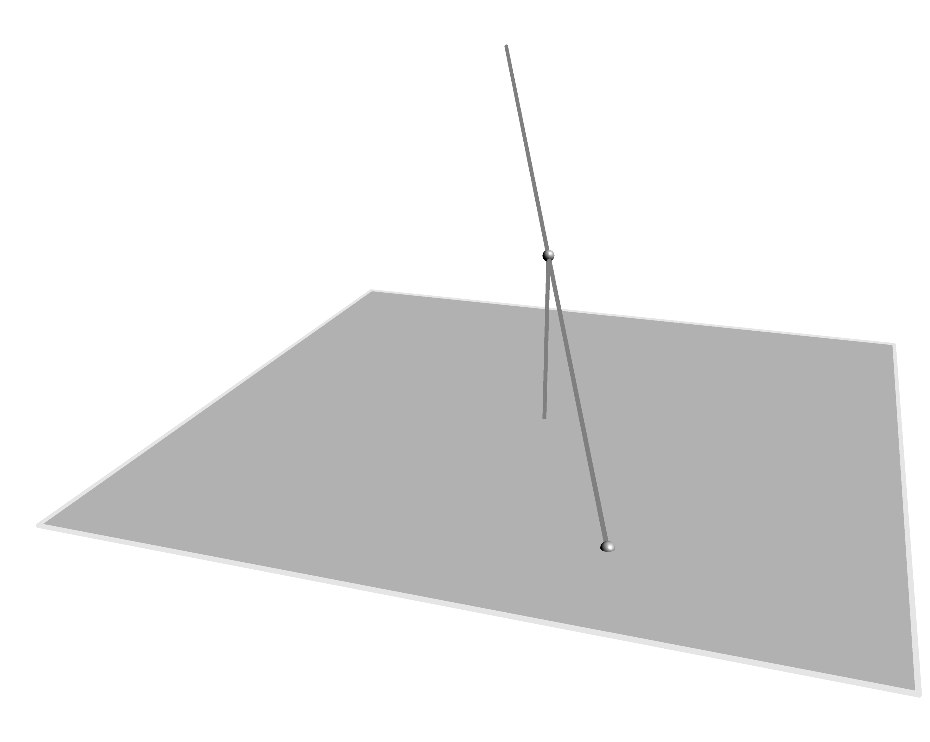
\includegraphics[width=5cm]{above-the-plane-connect}
\end{center}
or it is parallel to the plane
\begin{center}
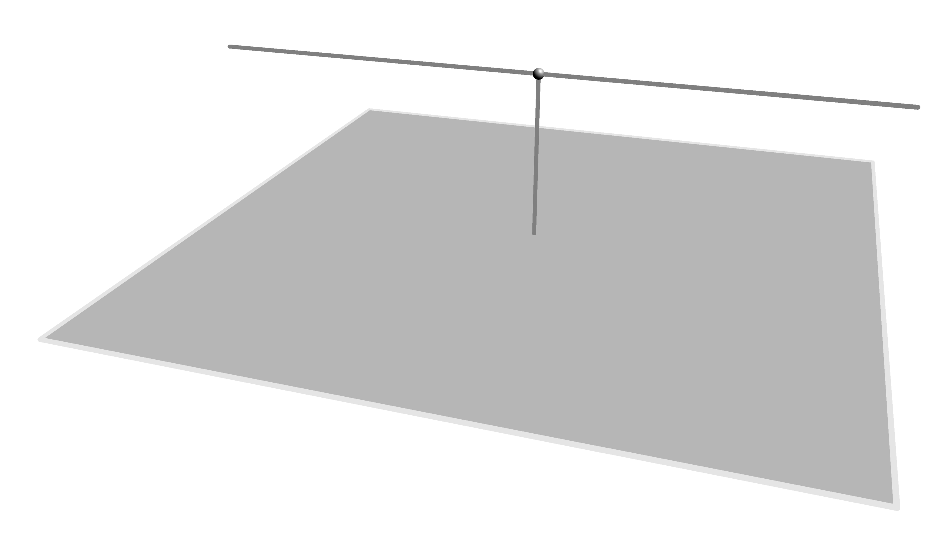
\includegraphics[width=5cm]{above-the-plane-off-to-infinity}
\end{center}
so that it is pointed along the direction of some train tracks (lines) in the plane, to some ``point at infinity''.
\begin{center}
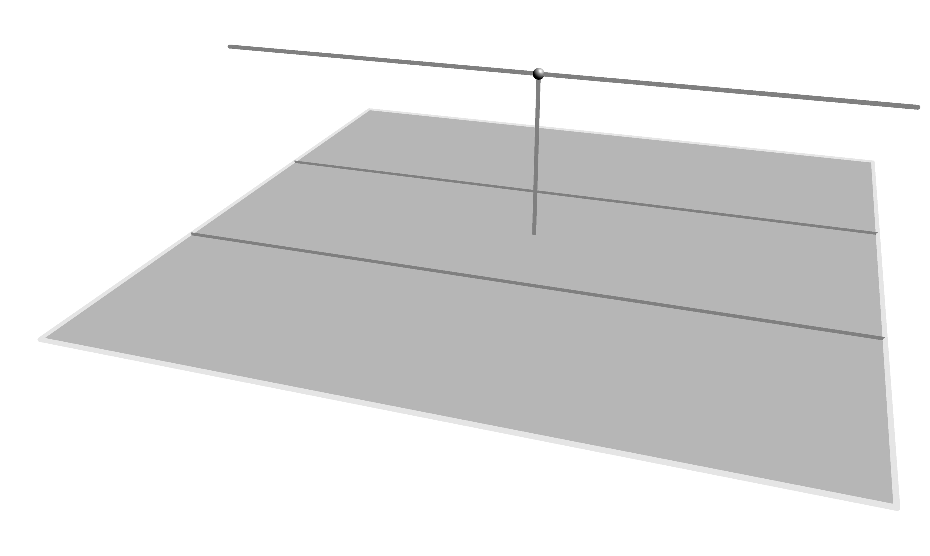
\includegraphics[width=5cm]{above-the-plane-3}
\end{center}
The points of the projective plane, finite points together with infinite points at infinity, are in 1-1 correspondence with lines through the vantage point.

This picture gives us a rigorous definition of points at infinity: the \emph{projective plane}\define{projective!plane} is the set of all lines through a chosen point of \(3\)-dimensional space, called the vantage point.
The \emph{points} of the projective plane (using this definition) are the lines through the vantage point.
The ``finite points'' are the lines not parallel to the horizontal plane.
The ``infinite points'' are the lines which are parallel the horizontal plane.
The set of finite points is the \emph{affine plane},\define{affine plane} which we think of as just the usual \(xy\)-plane.
The ``infinite points'' are precisely the horizontal lines, i.e. the lines in the horizontal plane through the vantage point. 
Being the set of lines in that plane, they constitute the projective line of that plane: the projective plane consists of an affine plane of finite points, and a projective line of points at infinity.

The \emph{lines}\define{projective!line}, also called \emph{projective lines}, of the projective plane we define to mean the planes through the vantage point.
\begin{center}
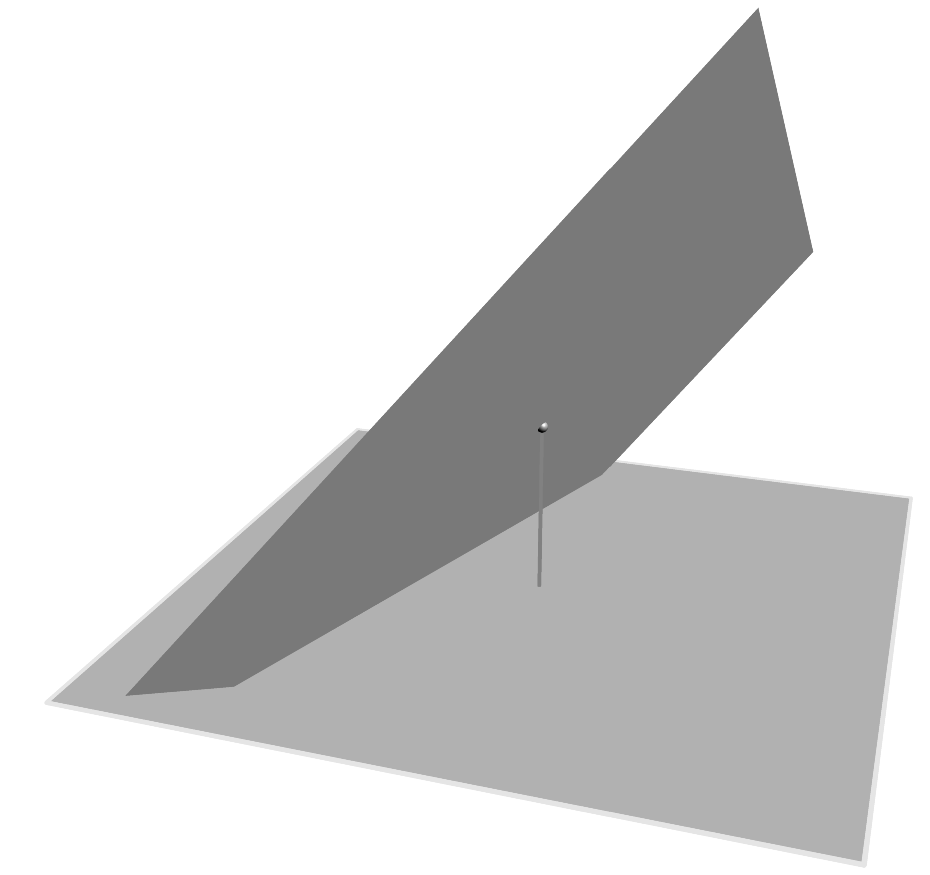
\includegraphics[width=5cm]{above-the-plane-projective-line}
\end{center}
\begin{problem}{projective.plane:join.points}
Prove that any two distinct points in the projective plane lie on a unique line.
\end{problem}
\begin{answer}{projective.plane:join.points}
A point of the projective plane is precisely a line through the vantage point in \(3\)-dimensional space \(\R{3}\).
A pair of distinct points in the projective plane is a pair of distinct lines through the vantage point.
Take the vantage point to be the origin, for simplicity of notation.
Clearly these lines span a unique plane in \(\R{3}\), i.e. the two points in the projective plane lie in a unique projective line.
\end{answer}
\begin{problem}{projective.plane:intersecting.lines}
Prove that any two distinct lines meet at a unique point. (Note how strange this is compared to usual plane geometry: there are no parallel lines in the projective plane.)
\end{problem}
\begin{answer}{projective.plane:intersecting.lines}
Our two lines in the projective plane are precisely two planes through the vantage point in our \(3\)-dimensional space \(\R{3}\).
Take the vantage point to be the origin, for simplicity of notation.
The intersection of linear subspaces is a linear subspace.
The dimension of a linear subspace is smaller than that of any linear subspace containing it, unless the two linear subspaces are equal.
So these planes intersect in a plane (if they are equal), or in a line, or just at the origin.
We wish to rule out this last possibility.
The dimension formula from linear algebra says that any two linear subspaces \(V,W\) satisfy
\[
\dim*{V+W}+\dim*{V\cap W}=\dim{V}+\dim{W}.
\]
Our planes have dimension \(2\), and sit in \(\R{3}\), which has dimension \(3\), so
\[
3+\dim*{V\cap W}\ge\dim*{V+W}+\dim*{V\cap W}=2+2.
\]
So \(\dim*{V\cap W}\ge 1\), i.e. our planes meet along a line or else they are equal.
\end{answer}

\section{Homogeneous coordinates}
We can make this more explicit by writing each point of \(3\)-dimensional space \(\R{3}\) as a triple
\[
\begin{pmatrix}
x\\
y\\
z
\end{pmatrix}
\]
and sometimes as \((x,y,z)\) to save space in writing.
Take the vantage point to be the origin.
Draw the horizontal plane in our pictures above not as the usual \(xy\)-plane, but as the plane \(z=1\).
Any linear change of the \(3\) variables \(x,y,z\) takes lines (and planes) through the origin to one another: there are more symmetries of the projective plane than we have ever encountered in the affine plane.

Every point of \(3\)-dimensional space not at the origin lies on a unique line through the origin.
So every point \((x,y,z)\) with not all of \(x,y,z\) zero lines on a unique line through the origin.
The points of this line are precisely the rescalings \((tx,ty,tz)\) of that point.
So each point of the projective plane can be written as a triple \((x,y,z)\), not all zero, and two such triples represent the same point just when each is a rescaling of the other.
Denote such a point with square brackets:
\[
\begin{bmatrix}
x\\
y\\
z
\end{bmatrix}
\]
and sometimes as \([x,y,z]\) to save space in writing.
For example, the point \([3,1,2]\) of the projective plane means the line through the origin consisting of the points of the form \((3t,t,2t)\) for all values of a variable \(t\), including \((3,1,2)\), \((3 \cdot 2, 1 \cdot 2, 2 \cdot 2)\), \((-3,-1,-2)\), and so on.
We write this as:
\[
[3,1,2]=[3 \cdot 2, 1 \cdot 2, 2 \cdot 2]=[-3,-1,-2].
\]
The coordinates \(x,y,z\) are the \emph{homogeneous coordinates}\define{homogeneous!coordinates}\define{coordinates!homogeneous} of a point \([x,y,z]\) of the projective plane.

In our pictures, we drew a horizontal below the vantage point, but it is more traditional to take the plane to be \(z=1\), above the vantage point \((x,y,z)=(0,0,0)\). 
The \emph{affine plane} is just the usual \(xy\) plane, but identified either with the plane \(z=1\), or with the subset of the projective plane given by points \([x,y,1]\).

\section{Linear transformations and projective transformations}
The roles of \(x,y,z\) are all the same now, and we can see that any linear change of variables of \(x,y,z\) takes the points of the projective plane to one another, and takes the lines of the projective plane to one another.
Each linear change of variables is represented by an invertible matrix
\[
A=
\begin{pmatrix}
a_{00} & a_{01} & a_{02} \\
a_{10} & a_{11} & a_{12} \\
a_{20} & a_{21} & a_{22}
\end{pmatrix}.
\]
Following convention, we often label our variables \((x,y,z)\) also as \((x_0,x_1,x_2)\), so label our matrix columns using \(0,1,2\) rather than \(1,2,3\).
Such a matrix takes a point \(p=[x,y,z]\) of the plane to the point \(q=[X,Y,Z]\) where
\[
\begin{pmatrix}
X \\
Y \\
Z
\end{pmatrix}
=
A
\begin{pmatrix}
x \\
y \\
z
\end{pmatrix}.
\]
We denote this relation as \(q=[A]p\) and call \([A]\) a \emph{projective transformation}\define{projective!transformation}.
\begin{problem}{projective.plane:permut}
Prove that the points of the projective plane are permuted by the projective transformations, as are the projective lines.
\end{problem}
\begin{problem}{projective.plane:mult}
Prove that for any invertible \(3 \times 3\) matrices \(A\) and \(B\), \([AB]=[A][B]\), i.e. we carry out the transformation of lines through the origin by carrying out the multiplications by the matrices.
\end{problem}
\begin{problem}{projective.plane:scaling.matrices}
Suppose that \(A\) is a square matrix which rescales every nonzero vector by a scalar, i.e. \(Ax=\lambda(x)x\) for some number \(\lambda(x)\), for every vector \(x \ne 0\). Prove that \(\lambda(x)\) is a constant scalar independent of \(x\), and \(A=\lambda I\) is a constant multiple of the identity matrix.
\end{problem}
\begin{answer}{projective.plane:scaling.matrices}
Suppose that \(A\) is \(n \times n\).
If \(n=1\) then every square matrix is a constant scalar, so suppose that \(n \ge 2\).
Write our vectors as \(x=\sum_j x_j e_j\) in the standard basis of \(\R{n}\) and calculate
\begin{align*}
Ax
&=
\lambda\of{x} x,
\\
&=
\sum_j \lambda\of{x} x_j e_j,
\\
&=
\sum_j x_j ge_j,
\\
&=
\sum_j x_j \lambda\of{e_j} e_j.
\end{align*}
So for any \(x\) with \(x_j\ne 0\), we have \(\lambda(x)=\lambda\of{e_j}\).
In particular, if \(x=e_1+e_2+\dots+e_n\), we have 
\[
\lambda\of{e_1}=\dots=\lambda\of{e_n}.
\]
So if \(x\ne 0\) then \(\lambda(x)=\lambda\of{e_1}\).
So \(\lambda\) is a constant.
\end{answer}
\begin{problem}{projective.plane:aut.gl}
Prove that two projective transformations \([A],[B]\) have precisely the same effect on all points \([x,y,z]\) of the projective plane just when the matrices agree up to a constant \(B=\lambda A\), some number \(\lambda \ne 0\).
\end{problem}
\begin{answer}{projective.plane:aut.gl}
Let \(C\defeq B^{-1}A\), so that \([C]=[B]^{-1}[A]\) and \([C]\) fixes every point of the projective plane just when \(C\) rescales every vector in \(\R{3}\) by  a scalar.
\end{answer}

\section{Arbitrary fields}
Over any field \(k\), in ``\(3\)-dimensional space'' \(k^3\), the line through two points 
\[
p=
\begin{pmatrix}
x \\
y \\
z
\end{pmatrix},
q=
\begin{pmatrix}
X \\
Y \\
Z
\end{pmatrix}
\]
is just the set of all points \(tp+(1-t)q\) for \(t\) in \(k\).
The \emph{projective plane}\define{projective!plane}, denoted \(\Proj^2_k\),\Notation{P2k}{\Proj^2_k}{projective plane over a field \(k\)} is the set of lines through the origin in \(k^3\); denoted \(\Proj^2\) if the field \(k\) is left implicit.
\begin{problem}{proj.plane}
Explain why \(\Proj^2_k=k^2\cup\Proj^1_k\), and use this to count the number of points of the projective plane over a finite field \(k\) with \(d\) elements.
\end{problem}

\section{Example: the Fano plane}
Let \(k\defeq \Zmod{2}\); the \emph{Fano plane}\define{Fano plane}\define{plane!Fano} is the projective plane \(\Proj^2_k\).
Each point is \([x,y,z]\) with \(x,y,z\) in \(k\) not all zero, defined up to rescaling them together.
But the only scalar you can use to rescale with is \(1\), since \(k=\Set{0,1}\).
Therefore we can just write \([x,y,z]\) as \((x,y,z)\).
Taking all possibilities for \(x,y,z\) from \(k\), not all zero, we get 7 points
\[
\begin{bmatrix}
1 \\
0 \\
0
\end{bmatrix},
\begin{bmatrix}
0 \\
1 \\
0
\end{bmatrix},
\begin{bmatrix}
1 \\
1 \\
0
\end{bmatrix},
\begin{bmatrix}
0 \\
0 \\
1
\end{bmatrix},
\begin{bmatrix}
1 \\
0 \\
1
\end{bmatrix},
\begin{bmatrix}
0 \\
1 \\
1
\end{bmatrix},
\begin{bmatrix}
1 \\
1 \\
1
\end{bmatrix},
\]
corresponding to the numbers \(1,2, \dots, 7\) written in base \(2\).

We can also draw this diagram as a cube; for each point, you draw the corresponding point in \(\R{3}\) with the same coordinates:
\begin{center}
\newcommand{\Depth}{1}
\newcommand{\Height}{1}
\newcommand{\Width}{1}
\tdplotsetmaincoords{70}{110}
\begin{tikzpicture}[tdplot_main_coords]
\coordinate (0) at (0,0,0);
\coordinate (1) at (\Depth,0,\Height);
\coordinate (2) at (\Depth,\Width,0);
\coordinate (3) at (0,\Width,\Height);
\coordinate (4) at (\Depth,\Width,\Height);
\coordinate (5) at (0,\Width,0);
\coordinate (6) at (0,0,\Height);
\coordinate (7) at (\Depth,0,0);

\draw[gray!10,fill=gray!10] (0) -- (6) -- (1) -- (7) -- cycle;% Left Face
\draw[gray!10,fill=gray!30] (0) -- (7) -- (2) -- (5) -- cycle;% Bottom Face
\draw[gray!10,fill=gray!40] (0) -- (6) -- (3) -- (5) -- cycle;% Back Face
\draw[gray!10,fill=gray!20,opacity=0.6] (1) -- (4) -- (2) -- (7) -- cycle;% Front Face
\draw[gray!10,fill=gray!20,opacity=0.8] (1) -- (4) -- (3) -- (6) -- cycle;% Top Face
\draw[gray!10,fill=gray!20,opacity=0.8] (4) -- (3) -- (5) -- (2) -- cycle;% Right Face

\node at (1) {\small\(6\)};
\node at (2) {\small\(3\)};
\node at (3) {\small\(5\)};
\node at (4) {\small\(7\)};
\node at (5) {\small\(1\)};
\node at (6) {\small\(4\)};
\node at (7) {\small\(2\)};

%% Following is for debugging purposes so you can see where the points are
%% These are last so that they show up on top
%\foreach \xy in {O, A, B, C, D, E, F, G}{
%    \node at (\xy) {\xy};
%}
\end{tikzpicture}
\end{center}
with one vertex not marked; the unmarked vertex is at the origin, so doesn't represent any point of the Fano plane.
Every line in the Fano plane has three vertices.
Take two numbers from 1 to 7, say \(1, 5\), and write out their binary digits under one another:
\[
\begin{array}{@{}c@{}c@{}c@{}}
0&0&1\\
1&0&1
\end{array}.
\]
Look at these as vectors in \(k^3\), so add them without carrying digits:
\[
\begin{array}{@{}c@{}c@{}c@{}}
0&0&1\\
1&0&1\\ \midrule
1&0&0
\end{array}
\]
The sum vector lies on the same line in the Fano plane, giving the lines:
\begin{center}
\newcommand{\Depth}{1}
\newcommand{\Height}{1}
\newcommand{\Width}{1}
\tdplotsetmaincoords{70}{110}
\begin{tikzpicture}[tdplot_main_coords]%Highlight the bottom
\coordinate (0) at (0,0,0);
\coordinate (1) at (\Depth,0,\Height);
\coordinate (2) at (\Depth,\Width,0);
\coordinate (3) at (0,\Width,\Height);
\coordinate (4) at (\Depth,\Width,\Height);
\coordinate (5) at (0,\Width,0);
\coordinate (6) at (0,0,\Height);
\coordinate (7) at (\Depth,0,0);
%

\draw[gray!10,fill=gray!10] (0) -- (6) -- (1) -- (7) -- cycle;% Left Face
\draw[gray!10,fill=gray!110] (0) -- (7) -- (2) -- (5) -- cycle;% Bottom Face
\draw[gray!10,fill=gray!40] (0) -- (6) -- (3) -- (5) -- cycle;% Back Face
\draw[gray!10,fill=gray!20,opacity=0.6] (1) -- (4) -- (2) -- (7) -- cycle;% Front Face
\draw[gray!10,fill=gray!20,opacity=0.8] (1) -- (4) -- (3) -- (6) -- cycle;% Top Face
\draw[gray!10,fill=gray!20,opacity=0.8] (4) -- (3) -- (5) -- (2) -- cycle;% Right Face

\node at (1) {\small\(6\)};
\node at (2) {\small\(3\)};
\node at (3) {\small\(5\)};
\node at (4) {\small\(7\)};
\node at (5) {\small\(1\)};
\node at (6) {\small\(4\)};
\node at (7) {\small\(2\)};

%% Following is for debugging purposes so you can see where the points are
%% These are last so that they show up on top
%\foreach \xy in {O, A, B, C, D, E, F, G}{
%    \node at (\xy) {\xy};
%}
\end{tikzpicture}
\begin{tikzpicture}[tdplot_main_coords]%Highlight the left
\coordinate (0) at (0,0,0);
\coordinate (1) at (\Depth,0,\Height);
\coordinate (2) at (\Depth,\Width,0);
\coordinate (3) at (0,\Width,\Height);
\coordinate (4) at (\Depth,\Width,\Height);
\coordinate (5) at (0,\Width,0);
\coordinate (6) at (0,0,\Height);
\coordinate (7) at (\Depth,0,0);
%

\draw[gray!10,fill=gray!90] (0) -- (6) -- (1) -- (7) -- cycle;% Left Face
\draw[gray!10,fill=gray!30] (0) -- (7) -- (2) -- (5) -- cycle;% Bottom Face
\draw[gray!10,fill=gray!40] (0) -- (6) -- (3) -- (5) -- cycle;% Back Face
\draw[gray!10,fill=gray!20,opacity=0.6] (1) -- (4) -- (2) -- (7) -- cycle;% Front Face
\draw[gray!10,fill=gray!20,opacity=0.8] (1) -- (4) -- (3) -- (6) -- cycle;% Top Face
\draw[gray!10,fill=gray!20,opacity=0.8] (4) -- (3) -- (5) -- (2) -- cycle;% Right Face

\node at (1) {\small\(6\)};
\node at (2) {\small\(3\)};
\node at (3) {\small\(5\)};
\node at (4) {\small\(7\)};
\node at (5) {\small\(1\)};
\node at (6) {\small\(4\)};
\node at (7) {\small\(2\)};

%% Following is for debugging purposes so you can see where the points are
%% These are last so that they show up on top
%\foreach \xy in {O, A, B, C, D, E, F, G}{
%    \node at (\xy) {\xy};
%}
\end{tikzpicture}
\begin{tikzpicture}[tdplot_main_coords]%Highlight back face
\coordinate (0) at (0,0,0);
\coordinate (1) at (\Depth,0,\Height);
\coordinate (2) at (\Depth,\Width,0);
\coordinate (3) at (0,\Width,\Height);
\coordinate (4) at (\Depth,\Width,\Height);
\coordinate (5) at (0,\Width,0);
\coordinate (6) at (0,0,\Height);
\coordinate (7) at (\Depth,0,0);
%

\draw[gray!10,fill=gray!10] (0) -- (6) -- (1) -- (7) -- cycle;% Left Face
\draw[gray!10,fill=gray!30] (0) -- (7) -- (2) -- (5) -- cycle;% Bottom Face
\draw[gray!10,fill=gray!120] (0) -- (6) -- (3) -- (5) -- cycle;% Back Face
\draw[gray!10,fill=gray!20,opacity=0.6] (1) -- (4) -- (2) -- (7) -- cycle;% Front Face
\draw[gray!10,fill=gray!20,opacity=0.8] (1) -- (4) -- (3) -- (6) -- cycle;% Top Face
\draw[gray!10,fill=gray!20,opacity=0.8] (4) -- (3) -- (5) -- (2) -- cycle;% Right Face

\node at (1) {\small\(6\)};
\node at (2) {\small\(3\)};
\node at (3) {\small\(5\)};
\node at (4) {\small\(7\)};
\node at (5) {\small\(1\)};
\node at (6) {\small\(4\)};
\node at (7) {\small\(2\)};

%% Following is for debugging purposes so you can see where the points are
%% These are last so that they show up on top
%\foreach \xy in {O, A, B, C, D, E, F, G}{
%    \node at (\xy) {\xy};
%}
\end{tikzpicture}
\begin{tikzpicture}[tdplot_main_coords]
\coordinate (0) at (0,0,0);
\coordinate (1) at (\Depth,0,\Height);
\coordinate (2) at (\Depth,\Width,0);
\coordinate (3) at (0,\Width,\Height);
\coordinate (4) at (\Depth,\Width,\Height);
\coordinate (5) at (0,\Width,0);
\coordinate (6) at (0,0,\Height);
\coordinate (7) at (\Depth,0,0);
%

\draw[gray!10,fill=gray!10] (0) -- (6) -- (1) -- (7) -- cycle;% Left Face
\draw[gray!10,fill=gray!30] (0) -- (7) -- (2) -- (5) -- cycle;% Bottom Face
\draw[gray!10,fill=gray!40] (0) -- (6) -- (3) -- (5) -- cycle;% Back Face
\draw[gray!10,fill=gray!20,opacity=0.6] (1) -- (4) -- (2) -- (7) -- cycle;% Front Face
\draw[gray!10,fill=gray!20,opacity=0.8] (1) -- (4) -- (3) -- (6) -- cycle;% Top Face
\draw[gray!10,fill=gray!20,opacity=0.8] (4) -- (3) -- (5) -- (2) -- cycle;% Right Face

\draw[gray!10,fill=gray!80,opacity=0.8] (0) -- (6) -- (4) -- (2) -- cycle;

\node at (1) {\small\(6\)};
\node at (2) {\small\(3\)};
\node at (3) {\small\(5\)};
\node at (4) {\small\(7\)};
\node at (5) {\small\(1\)};
\node at (6) {\small\(4\)};
\node at (7) {\small\(2\)};

%% Following is for debugging purposes so you can see where the points are
%% These are last so that they show up on top
%\foreach \xy in {O, A, B, C, D, E, F, G}{
%    \node at (\xy) {\xy};
%}
\end{tikzpicture}
\begin{tikzpicture}[tdplot_main_coords]
\coordinate (0) at (0,0,0);
\coordinate (1) at (\Depth,0,\Height);
\coordinate (2) at (\Depth,\Width,0);
\coordinate (3) at (0,\Width,\Height);
\coordinate (4) at (\Depth,\Width,\Height);
\coordinate (5) at (0,\Width,0);
\coordinate (6) at (0,0,\Height);
\coordinate (7) at (\Depth,0,0);
%

\draw[gray!10,fill=gray!10] (0) -- (6) -- (1) -- (7) -- cycle;% Left Face
\draw[gray!10,fill=gray!30] (0) -- (7) -- (2) -- (5) -- cycle;% Bottom Face
\draw[gray!10,fill=gray!40] (0) -- (6) -- (3) -- (5) -- cycle;% Back Face
\draw[gray!10,fill=gray!20,opacity=0.6] (1) -- (4) -- (2) -- (7) -- cycle;% Front Face
\draw[gray!10,fill=gray!20,opacity=0.8] (1) -- (4) -- (3) -- (6) -- cycle;% Top Face
\draw[gray!10,fill=gray!20,opacity=0.8] (4) -- (3) -- (5) -- (2) -- cycle;% Right Face

\draw[gray!10,fill=gray!80,opacity=0.8] (0) -- (1) -- (4) -- (5) -- cycle;

\node at (1) {\small\(6\)};
\node at (2) {\small\(3\)};
\node at (3) {\small\(5\)};
\node at (4) {\small\(7\)};
\node at (5) {\small\(1\)};
\node at (6) {\small\(4\)};
\node at (7) {\small\(2\)};

%% Following is for debugging purposes so you can see where the points are
%% These are last so that they show up on top
%\foreach \xy in {O, A, B, C, D, E, F, G}{
%    \node at (\xy) {\xy};
%}
\end{tikzpicture}
{
\tdplotsetmaincoords{50}{110}
\begin{tikzpicture}[tdplot_main_coords]
\coordinate (0) at (0,0,0);
\coordinate (1) at (\Depth,0,\Height);
\coordinate (2) at (\Depth,\Width,0);
\coordinate (3) at (0,\Width,\Height);
\coordinate (4) at (\Depth,\Width,\Height);
\coordinate (5) at (0,\Width,0);
\coordinate (6) at (0,0,\Height);
\coordinate (7) at (\Depth,0,0);

\draw[gray!10,fill=gray!10] (0) -- (6) -- (1) -- (7) -- cycle;% Left Face
\draw[gray!10,fill=gray!30] (0) -- (7) -- (2) -- (5) -- cycle;% Bottom Face
\draw[gray!10,fill=gray!40] (0) -- (6) -- (3) -- (5) -- cycle;% Back Face
\draw[gray!10,fill=gray!20,opacity=0.6] (1) -- (4) -- (2) -- (7) -- cycle;% Front Face
\draw[gray!10,fill=gray!20,opacity=0.8] (1) -- (4) -- (3) -- (6) -- cycle;% Top Face
\draw[gray!10,fill=gray!20,opacity=0.8] (4) -- (3) -- (5) -- (2) -- cycle;% Right Face

\draw[gray!10,fill=gray!80,opacity=0.8] (0) -- (7) -- (4) -- (3) -- cycle;

\node at (1) {\small\(6\)};
\node at (2) {\small\(3\)};
\node at (3) {\small\(5\)};
\node at (4) {\small\(7\)};
\node at (5) {\small\(1\)};
\node at (6) {\small\(4\)};
\node at (7) {\small\(2\)};

%% Following is for debugging purposes so you can see where the points are
%% These are last so that they show up on top
%\foreach \xy in {O, A, B, C, D, E, F, G}{
%    \node at (\xy) {\xy};
%}
\end{tikzpicture}
}
\begin{tikzpicture}[tdplot_main_coords]
\coordinate (0) at (0,0,0);
\coordinate (1) at (\Depth,0,\Height);
\coordinate (2) at (\Depth,\Width,0);
\coordinate (3) at (0,\Width,\Height);
\coordinate (4) at (\Depth,\Width,\Height);
\coordinate (5) at (0,\Width,0);
\coordinate (6) at (0,0,\Height);
\coordinate (7) at (\Depth,0,0);

\draw[gray!10,fill=gray!10] (0) -- (6) -- (1) -- (7) -- cycle;% Left Face
\draw[gray!10,fill=gray!30] (0) -- (7) -- (2) -- (5) -- cycle;% Bottom Face
\draw[gray!10,fill=gray!40] (0) -- (6) -- (3) -- (5) -- cycle;% Back Face
\draw[gray!10,fill=gray!20,opacity=0.6] (1) -- (4) -- (2) -- (7) -- cycle;% Front Face
\draw[gray!10,fill=gray!20,opacity=0.8] (1) -- (4) -- (3) -- (6) -- cycle;% Top Face
\draw[gray!10,fill=gray!20,opacity=0.8] (4) -- (3) -- (5) -- (2) -- cycle;% Right Face

\draw[gray!10,fill=gray!80,opacity=0.8] (1) -- (3) -- (2) -- cycle;

\node at (1) {\small\(6\)};
\node at (2) {\small\(3\)};
\node at (3) {\small\(5\)};
%\node at (4) {\small\(7\)};
\node at (5) {\small\(1\)};
\node at (6) {\small\(4\)};
\node at (7) {\small\(2\)};
\end{tikzpicture}
\end{center}


\section{Projective space}
Similarly, \emph{projective space}\define{projective!space} \(\Proj^n_k\)\Notation{Pnk}{\Proj^n_k}{projective space over a field \(k\)} is the set of lines through the origin of \(k^{n+1}\), and a \emph{projective transformation}\define{projective!automorphism} of projective space is the result of applying an invertible square matrix to those lines.
Again, two invertible square matrices yield the same projective transformation just when they agree up to a scalar multiple, by the same proof.
We often denote \(\Proj^n_k\) simply as \(\Proj^n\) when the field \(k\) is not foremost in our thoughts.
Write each point of \(\Proj^n\) as
\[
[x]=\begin{bmatrix}x_0\\ x_1\\ \vdots\\ x_n\end{bmatrix}
\]
to mean the line through the origin and the vectors
\[
x=\begin{pmatrix}x_0\\ x_1\\ \vdots\\ x_n\end{pmatrix}
\]
of \(k^{n+1}\).

\section{Projective space and field extensions}
Consider a field extension \(k\subset K\).
Each point \([x]\) of \(\Proj^n_k\) has an associated point \([x]\) of \(\Proj^n_K\): we simply allow rescaling by any nonzero element of \(K\), i.e. the line in the sense of \(K\).
This maps \(\Proj^n_k\to\Proj^n_K\).
\begin{problem}{proj.plane:extend}
Prove that a point \([x]\) of \(\Proj^n_K\) arises via this map from a point of \(\Proj^n_k\) just when the ratios \(x_i/x_j\) are elements of \(k\), for any \(i,j=0,1,\dots,n\) for which \(x_j\ne 0\).
\end{problem}
\begin{problem}{proj.plane:extend.2}
Prove that this map is injective.
\end{problem}
Hence we can consider the points of \(\Proj^n_K\) to be the \(K\)-points of \(\Proj^n_k\).
\begin{problem}{proj.plane:affine.k}
Prove that each \emph{affine space}\define{affine space} \((x_i=1)\) in \(\Proj^n_k\) is precisely the set of \(k\)-points of the affine space \((x_i=1)\) in \(\Proj^n_K\).
\end{problem}
\begin{problem}{proj.plane:Gal}
Explain how the Galois group \(\Gal{k}{K}\) acts on \(\Proj^n_K\), leaving fixed all points of \(\Proj^n_k\).
\end{problem}

\section{Subspaces of projective spaces}
A \emph{subspace}\define{projective!subspace}\define{subspace!projective} of a projective space \(\Proj^n_k\) is the set of lines lying in some linear subspace \(V\subset k^{n+1}\); denote this subspace \(\Proj(V)\subset\Proj^n_k\).
The \emph{dimension} of \(\Proj(V)\) is defined to be one less than the dimension of \(V\).
Careful: we allow \(V=\set{0}\), but then define \(\Proj(V)\) to mean the empty set, which has ``dimension'' \(-1\).
Subspaces of various dimensions are called:
\[
\begin{array}{rl}
\toprule 
\text{dimension}&\text{type}\\
\cmidrule(r){1-1}\cmidrule(l){2-2}
-1 & \text{empty set}\\
0 & \text{point}\\
1 & \text{\emph{line} or \emph{projective line}}\define{line!projective}\define{projective!line}\\
2 & \text{\emph{plane} or \emph{projective plane}}\define{plane!projective}\define{projective!plane}\\
n-1 & \text{\emph{hyperplane} or \emph{projective hyperplane}}\define{projective!hyperplane}\define{hyperplane!projective}\\ \bottomrule
\end{array}
\]
\begin{problem}{proj.plane:intersect}
Suppose that \(X\) and \(Y\) are subspaces of a projective space \(\Proj^n\).
Why is \(X\cap Y\) also a subpace?
\end{problem}
\begin{problem}{proj.plane:intersect.2}
What are the possible dimensions of intersections of subspaces (of all possible dimensions) in \(\Proj^3\), up to projective transformations? In \(\Proj^4\)?
\end{problem}
For any subset \(S\subseteq\Proj^n\), let \(\left<S\right>\) be the smallest subspace containing \(S\), the \emph{span}\define{span} of \(S\).
\begin{problem}{proj.plane:spn}
Prove that \(\left<S\right>\) exists for any set \(S\subseteq\Proj^n\).
\end{problem}
\begin{problem}{proj.plane:dim}
Suppose that \(X\) and \(Y\) are subspaces of a projective space \(\Proj^n\).
Prove that
\[
\dim{\left<X,Y\right>}+\dim*{X\cap Y}=\dim{X}+\dim{Y}.
\]
\end{problem}
\begin{problem}{proj.plane:lines}
Prove that any two distinct points of any projective space lie on a unique line.
\end{problem}
\begin{problem}{proj.plane:project}
Suppose that \(X\) and \(Y\) are hyperplanes and \(p_0\) is a point not on either.
Prove that for each point \(x\in X\) there is a unique point \(y\in Y\) so that \(p_0,x\) and \(y\) lie on the same line, hence a map \(\map{\varphi}{X}{Y}\) defined by taking each point \(x\) to the point \(y\) on the same line through \(p_0\).
Prove that \(\varphi\) take every line in \(X\) to a line in \(Y\).
\end{problem}
\begingroup
% Commands for the discussion of Desargues's theorem:
% highest x value of any coordinate of any point in the picture:
\newcommand*{\maxX}{6}
% lowest x value of any coordinate of any point in the picture:
\newcommand*{\minX}{0.1}

\newcommand*{\AoneX}{2.99}
\newcommand*{\AoneY}{0}
\newcommand*{\Aone}{\AoneX,\AoneY}
\newcommand*{\AtwoX}{4.22}
\newcommand*{\AtwoY}{.6}
\newcommand*{\Atwo}{\AtwoX,\AtwoY}
\newcommand*{\AthreeX}{4.68}
\newcommand*{\AthreeY}{1.41}
\newcommand*{\Athree}{\AthreeX,\AthreeY}
\newcommand*{\PnoughtX}{4.05}
\newcommand*{\PnoughtY}{3.11}
\newcommand*{\Pnought}{\PnoughtX,\PnoughtY}
\newcommand*{\Tone}{1.5627}
\newcommand*{\Ttwo}{2.1116}
\newcommand*{\Tthree}{2.9353}

\newcommand*{\drawOrigin}
{
\coordinate (p) at (\Pnought){};
\DrawNode{p}
}

\newcommand*{\drawFirstTriangle}
{
\coordinate (a1) at (\Aone){};
\DrawNode{a1}
\coordinate (a2) at (\Atwo){};
\DrawNode{a2}
\coordinate (a3) at (\Athree){};
\DrawNode{a3}
\begin{scope}[on background layer]
\fill[shapeOne] (a1) -- (a2) -- (a3) -- cycle;
\end{scope}
}

\newcommand*{\Bone}{{\Tone*(\AoneX-\PnoughtX)+\PnoughtX},{\Tone*(\AoneY-\PnoughtY)+\PnoughtY}}
\newcommand*{\Btwo}{{\Ttwo*(\AtwoX-\PnoughtX)+\PnoughtX},{\Ttwo*(\AtwoY-\PnoughtY)+\PnoughtY}}
\newcommand*{\Bthree}{{\Tthree*(\AthreeX-\PnoughtX)+\PnoughtX},{\Tthree*(\AthreeY-\PnoughtY)+\PnoughtY}}

\newcommand*{\drawSecondTriangle}
{
\coordinate (b1) at (\Bone){};
\DrawNode{b1}
\coordinate (b2) at (\Btwo){};
\DrawNode{b2}
\coordinate (b3) at (\Bthree){};
\DrawNode{b3}
\begin{scope}[on background layer]
\fill[shapeTwo] (b1) -- (b2) -- (b3) -- cycle;
\end{scope}
}

\newcommand*{\connectVantageAndFirstTwoTriangles}
{
\begin{scope}[on background layer]
\draw[curveZero,very thick] (p) -- (a1) -- (b1);
\draw[curveZero,very thick] (p) -- (a2) -- (b2);
\draw[curveZero,very thick] (p) -- (a3) -- (b3);
\end{scope}
}

\newcommand*{\findFirstIntersection}
{
\coordinate (c1) at (intersection of a2--a3 and b2--b3) {};
}
\newcommand*{\findSecondIntersection}
{
\coordinate (c2) at (intersection of a1--a3 and b1--b3) {};
}
\newcommand*{\findThirdIntersection}
{
\coordinate (c3) at (intersection of a1--a2 and b1--b2) {};
}

\newcommand*{\findAllIntersections}
{
\findFirstIntersection
\findSecondIntersection
\findThirdIntersection
}

\newcommand*{\showFirstIntersectionPoint}
{
\DrawNode{c1}
}

\newcommand*{\showSecondIntersectionPoint}
{
\DrawNode{c2}
}

\newcommand*{\showThirdIntersectionPoint}
{
\DrawNode{c3}
}


\newcommand*{\showAllIntersectionPoints}
{
\showFirstIntersectionPoint
\showSecondIntersectionPoint
\showThirdIntersectionPoint
}

\newcommand*{\showHowFirstIntersectionIsConstructed}
{
\begin{scope}[on background layer]
\draw[curveOne,very thick] (a3) -- (c1); % line through c1
\draw[curveOne,very thick] (a2) -- (c1); % line through c1
\draw[curveOne,very thick] (b2) -- (c1); % line through c1
\draw[curveOne,very thick] (b3) -- (c1); % line through c1
\end{scope}
\showFirstIntersectionPoint
}

\newcommand*{\showHowSecondIntersectionIsConstructed}
{
\begin{scope}[on background layer]
\draw[curveTwo,very thick] (a3) -- (c2); % line through c2
\draw[curveTwo,very thick] (a1) -- (c2); % line through c2
\draw[curveTwo,very thick] (b1) -- (c2); % line through c2
\draw[curveTwo,very thick] (b3) -- (c2); % line through c2
\end{scope}
\showSecondIntersectionPoint
}

\newcommand*{\showHowThirdIntersectionIsConstructed}
{
\begin{scope}[on background layer]
\draw[curveThree,very thick] (a1) -- (c3); % line through c3
\draw[curveThree,very thick] (a2) -- (c3); % line through c3
\draw[curveThree,very thick] (b1) -- (c3); % line through c3
\draw[curveThree,very thick] (b2) -- (c3); % line through c3
\end{scope}
\showThirdIntersectionPoint
}

\newcommand*{\showHowAllIntersectionsAreConstructed}
{
\showHowFirstIntersectionIsConstructed
\showHowSecondIntersectionIsConstructed
\showHowThirdIntersectionIsConstructed
}

\newcommand*{\showTheLine}
{
\begin{scope}[on background layer]
\draw[curveZero,very thick] (c1) -- (c2);
\draw[curveZero,very thick] (c1) -- (c3);
\draw[curveZero,very thick] (c2) -- (c3);
\end{scope}
\showAllIntersectionPoints
}

\newcommand*{\showThirdTriangle}
{
\begin{scope}[on background layer]
\fill[
shapeThree,draw=curveThree,very thick
%green!50!gray,opacity=.1
] (c1) to[bend left=85] (c2) to[bend right=85] (c3) to[bend left=90] (c1);
\end{scope}
\showAllIntersectionPoints
}


\newcommand{\Desargue}[1]{%
\begin{center}
\begin{tikzpicture}
% Draw a strut to make all of the diagrams have the same width, so the same x coordinate in each diagram gives a point the same distant across the page.
\begin{scope}[on background layer]
\draw[white] (\minX,0) -- (\maxX,0); 
\end{scope}
\IfStrEqCase{#1}{%
{1}%
{%%
\drawOrigin
\drawFirstTriangle
}%%
{2}%
{%
\drawOrigin
\drawFirstTriangle
\drawSecondTriangle
\connectVantageAndFirstTwoTriangles
\drawFirstTriangle
\drawSecondTriangle
}%
{3}%
{%%
\drawOrigin
\drawFirstTriangle
\drawSecondTriangle
\findFirstIntersection
\showHowFirstIntersectionIsConstructed
}%%
{4}%
{%%
\drawOrigin
\drawFirstTriangle
\drawSecondTriangle
\findSecondIntersection
\showHowSecondIntersectionIsConstructed
}%%
{5}%
{%%
\drawOrigin
\drawFirstTriangle
\drawSecondTriangle
\findThirdIntersection
\showHowThirdIntersectionIsConstructed
}%%
{6}%
{%%
\drawOrigin
\drawFirstTriangle
\drawSecondTriangle
\findAllIntersections
\showTheLine
}%%
{7}%
{%%
\drawOrigin
\drawFirstTriangle
\drawSecondTriangle
\connectVantageAndFirstTwoTriangles
\findAllIntersections
\showHowAllIntersectionsAreConstructed
\showTheLine
}%%
{8}%
{%%
\drawOrigin
\drawFirstTriangle
\drawSecondTriangle
\connectVantageAndFirstTwoTriangles
\findAllIntersections
\showHowAllIntersectionsAreConstructed
\showThirdTriangle
}%%
{9}%
{%%
\drawFirstTriangle
\drawSecondTriangle
\findAllIntersections
\showHowAllIntersectionsAreConstructed
\showTheLine
}%%
{10}%
{%%
\drawFirstTriangle
\drawSecondTriangle
\findAllIntersections
\showHowAllIntersectionsAreConstructed
\showTheLine
\begin{scope}[on background layer]
\draw[opacity=0] (c1) -- ++(6cm,0) node[black] (c4) {\(c_4\)};
\draw[opacity=0] (c3) -- ++(6cm,0) node[brown] (c5) {\(c_5\)};
\fill[shapeZero,draw=curveZero] (c4.center) -- (c5.center) -- (c3.center) -- (c1.center) -- cycle;
\end{scope}
\begin{scope}[on background layer]
\draw[opacity=0] (c1) -- ++(6cm,4cm) node[black] (d1) {\(d_1\)};
\draw[opacity=0] (c3) -- ++(6cm,4cm) node[brown] (d3) {\(d_3\)};
\fill[shapeZero,draw=curveZero] (d1.center) -- (d3.center) -- (c3.center) -- (c1.center) -- cycle;
\end{scope}
}%%
}%% end IfStrEqCase
\end{tikzpicture}
\end{center}
}

\Desargue{2}
\endgroup
\begin{problem}{proj.plane:pts}
If \(k\) is a finite field with \(d\) elements, prove that the number of \(p\)-dimensional subspaces of \(\Proj^n_k\) is
\[
\frac{(d^{n+1}-1)(d^{n+1}-d)\dots(d^{n+1}-d^p)}{(d^{n+1}-1)(d^{n+1}-d)\dots(d^{p+1}-d^p)}.
\]
\end{problem}
\begin{problem*}{projective.plane:bases}
A \emph{basis}\define{basis} of the projective plane is a collection of \(4\) points \(p_0,p_1,p_2,p_3\), no three in the same line.
Prove that there is a basis, and that any two bases are identified by a unique projective transformation.
\end{problem*}
\begin{answer}{projective.plane:bases}
We turn the problem into linear algebra.
Each point \(p_i\) in our projective plane is some
\[
p_i=
\begin{bmatrix}
x_i\\
y_i\\
z_i
\end{bmatrix}
\]
line through the origin and some vector
\[
v_i=
\begin{pmatrix}
x_i\\
y_i\\
z_i
\end{pmatrix}.
\]
Any three of these four vectors \(v_0,v_1,v_2,v_3\) are linearly independent, i.e. don't lie in the same plane through the origin.
So \(v_1,v_2,v_3\) is a basis and we can somehow write
\[
v_0=c_1v_1+c_2v_2+c_3v_3,
\] 
for some \(c_1,c_2,c_3\) in our field.
If \(c_1=0\) then this is a linear relation
\[
v_0=c_2v_2+c_3v_3,
\]
between three of our vectors, so they are linearly independent, so they lie in a plane, so \(p_0,p_2,p_3\) lie in a projective line, a contradiction.
Hence \(c_1\ne 0\).
By the same argument, \(c_1,c_2,c_3\) are all nonzero.
We can replace \(v_1,v_2,v_3\) by \(c_1v_1,c_2v_2,c_3v_3\) if we like, so we can assume that \(1=c_1=c_2=c_3\):
\[
v_0=v_1+v_2+v_3.
\]
Say that \(v_0,v_1,v_2,v_3\) are \emph{normalized} if this equation holds.

Claim: a normalized set of vectors is unique up to rescaling all of them by the same factor.
Proof: Suppose that instead we had chosen some other normalized vectors, say \(v_0',v_1',v_2',v_3'\) with  each \(v_i'\) also in the line represented by \(p_i\).
So then \(v_i'=a_i v_i\) for some constants \(a_i\ne 0\).
Then 
\[
v_0=\frac{v_0'}{a_0}=\frac{v_1'+v_2'+v_3'}{a_0}=\frac{a_1}{a_0}v_0+\frac{a_2}{a_0}v_2+\frac{a_3}{a_0}v_3,
\]
but 
\[
v_0=v_1+v_2+v_3.
\]
Since \(v_1,v_2,v_3\) is a basis, expansion in a basis is unique, so
\[
a_0=a_1=a_2=a_3.
\]

Pick some normalized \(v_0,v_1,v_2,v_3\) for a basis \(p_0,p_1,p_2,p_3\) and \(w_0,w_1,w_2,w_3\) for a basis \(q_0,q_1,q_2,q_3\).
From linear algebra, we know that there is a unique invertible \(3\times 3\) matrix \(A\) which linearly transforms vectors by \(x\mapsto Ax\), taking \(v_1,v_2,v_3\) to \(w_1,w_2,w_3\).
But then
\[
v_0=v_1+v_2+v_3
\]
ensures that
\[
Av_0=Av_1+Av_2+Av_3=w_1+w_2+w_3=w_0.
\]
So \([A]\) takes \(p_0,p_1,p_2,p_3\) to \(q_0,q_1,q_2,q_3\).
\end{answer}
\begin{theorem}[Pappus]\label{theorem:Pappus}\define{theorem!Pappus}\define{Pappus's theorem}
Take points \(p,q,r,p',q',r'\) be points of the projective plane.
Suppose that 
\[
p\ne q', p\ne r', 
\]
and all inequalities obtained from these by cyclically permuting labels \(p,q,r\).
Let
\begin{align*}
p''&=qr'\cap q'r, \\
q''&=rp'\cap r'p, \\
r''&=pq'\cap p'q.
\end{align*} 
If \(p,q,r\) are collinear, and \(p',q',r'\) are colinear, then \(p'',q'',r''\) are collinear.
\end{theorem}
\begin{proof}
Suppose that \(p,q,r',q'\) is not a basis.
Then two of the points \(p'',q'',r''\) coincide and Pappus's theorem is trivial.
Suppose that \(p,q,r',q'\) is a basis.
By problem~\vref{problem:projective.plane:bases} we can arrange that these are the standard basis:
\[
p,q,r',q'=[1,0,0], [0,1,0], [0,0,1], [1,1,1].
\]
\begin{problem}{projective.plane:Pappus}
Finish the proof of Pappus's theorem by linear algebra.
\end{problem}
\end{proof}
